
\documentclass[border=5pt]{standalone}
\usepackage{tikz}
\usetikzlibrary{arrows.meta, backgrounds, decorations.pathreplacing, fit, shapes.geometric}
\usepackage{amsmath, amssymb}

\definecolor{colglobal}{HTML}{4F6D7A}
\definecolor{colpop}{HTML}{8F5A83}
\definecolor{coldet}{HTML}{1F9D8A}
\definecolor{colsample}{HTML}{8A4F7D}
\definecolor{coldata}{HTML}{D8D8D8}

\tikzset{
    dag node/.style={
        draw=black!70, semithick, align=center,
        font=\scriptsize, inner sep=2.3pt,
    },
    global/.style={dag node, rectangle, rounded corners=2pt,
        minimum width=1.75cm, minimum height=0.56cm, fill=colglobal!10},
    selection/.style={dag node, rectangle, dashed, draw=black!60,
        fill=white, minimum width=1.85cm, minimum height=0.56cm},
    popdist/.style={dag node, rectangle, draw=colpop!85!black,
        dashed, fill=colpop!8, minimum height=0.66cm,
        text width=1.95cm, inner sep=1.3pt},
    latent/.style={dag node, ellipse, fill=white,
        minimum width=1.45cm, minimum height=0.58cm},
    det/.style={dag node, diamond, aspect=2.35, draw=coldet!85!black,
        fill=coldet!8, inner xsep=1pt, inner ysep=1pt},
    sample/.style={dag node, rectangle, draw=colsample!85!black,
        fill=colsample!8, minimum height=0.62cm,
        text width=1.95cm, inner sep=1.3pt},
    data/.style={dag node, rectangle, very thick, fill=coldata,
        minimum width=1.5cm, minimum height=0.56cm},
    conditioned/.style={data, double, double distance=1pt},
    plate/.style={draw=black!55, rounded corners=5pt, dashed,
        inner xsep=9pt, inner ysep=10pt},
    level label/.style={font=\scriptsize, text=black!70},
    legend text/.style={font=\scriptsize, anchor=west},
    dag edge/.style={-{Stealth[length=3pt, width=2.5pt]}, thin,
        draw=black!55},
    sel edge/.style={dag edge, draw=black!38},
}

\begin{document}
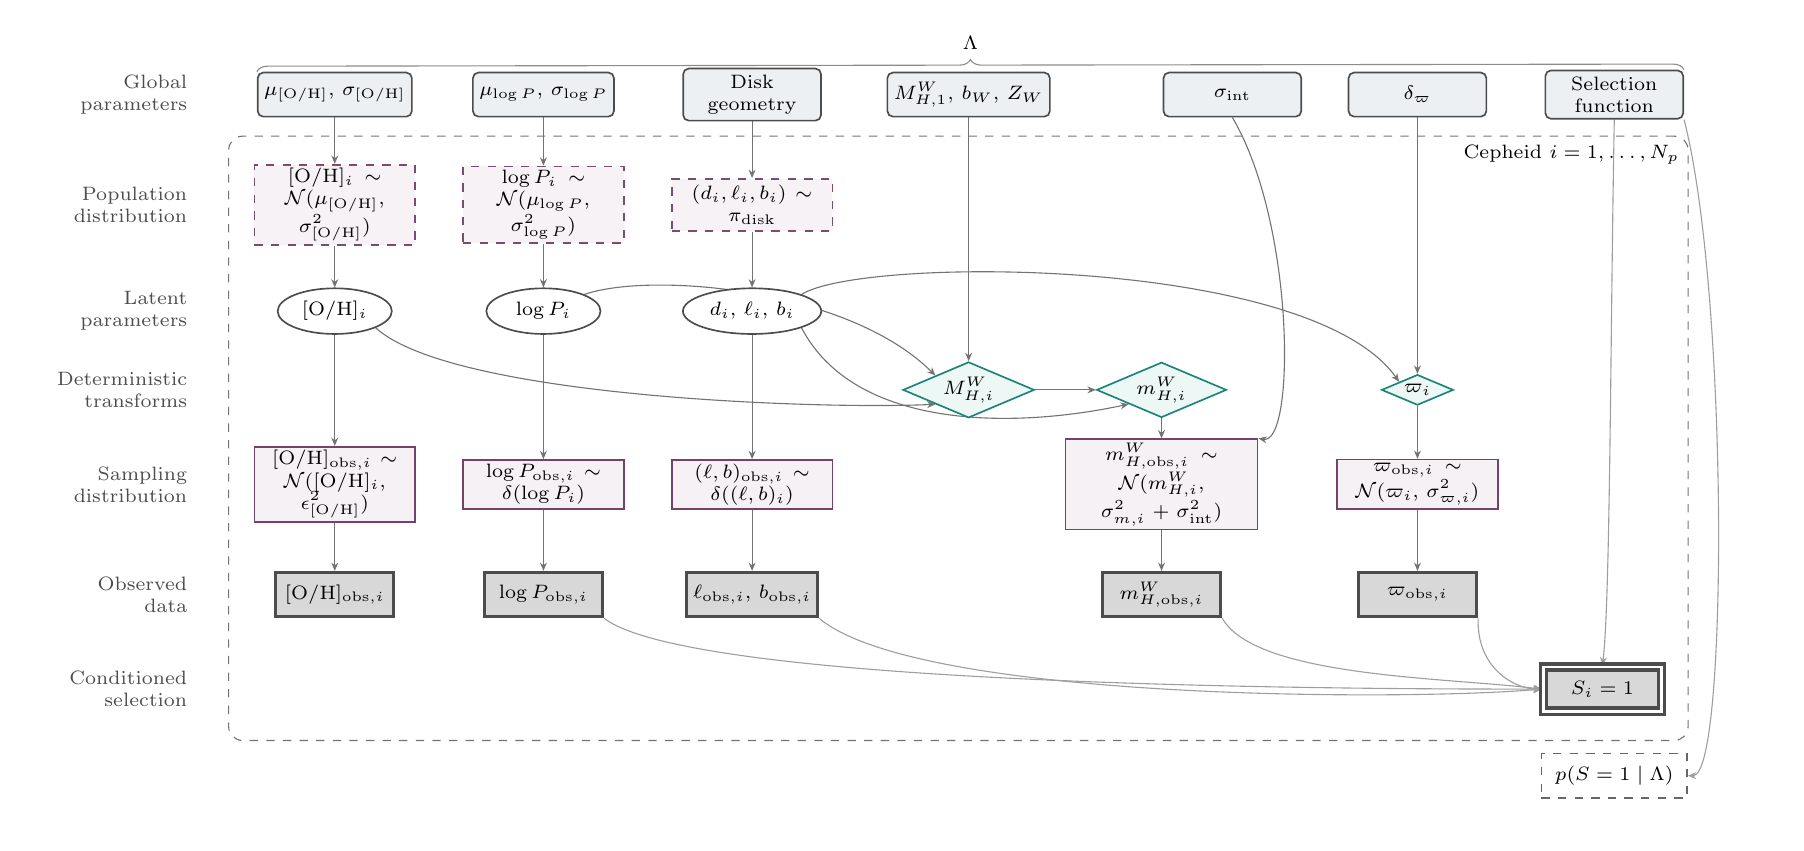
\begin{tikzpicture}

\useasboundingbox (-3.30, -2.25) rectangle (18.90, 7.85);

% ===== LEVEL LABELS =====
\node[level label, anchor=east, align=right] at (-1.15, 7.00) {Global\\parameters};
\node[level label, anchor=east, align=right] at (-1.15, 5.60) {Population\\distribution};
\node[level label, anchor=east, align=right] at (-1.15, 4.25) {Latent\\parameters};
\node[level label, anchor=east, align=right] at (-1.15, 3.25) {Deterministic\\transforms};
\node[level label, anchor=east, align=right] at (-1.15, 2.05) {Sampling\\distribution};
\node[level label, anchor=east, align=right] at (-1.15, 0.65) {Observed\\data};
\node[level label, anchor=east, align=right] at (-1.15, -0.55) {Conditioned\\selection};

% ===== NODES =====
\node[global] (OHpop) at (0.60, 7.00) {$\mu_{[\mathrm{O/H}]},\,\sigma_{[\mathrm{O/H}]}$};
\node[global] (Ppop) at (3.25, 7.00) {$\mu_{\log P},\,\sigma_{\log P}$};
\node[global] (disk) at (5.90, 7.00) {Disk\\geometry};
\node[global] (PL) at (8.65, 7.00) {$M^{W}_{H,1},\,b_W,\,Z_W$};
\node[global] (sint) at (12.00, 7.00) {$\sigma_{\rm int}$};
\node[global] (dpi) at (14.35, 7.00) {$\delta_\varpi$};
\node[global] (selcuts) at (16.85, 7.00) {Selection\\function};
\node[popdist] (OHdist) at (0.60, 5.60) {$[\mathrm{O/H}]_i \sim$\\$\mathcal{N}(\mu_{[\mathrm{O/H}]},$\\$\sigma_{[\mathrm{O/H}]}^2)$};
\node[popdist] (Pdist) at (3.25, 5.60) {$\log P_i \sim$\\$\mathcal{N}(\mu_{\log P},$\\$\sigma_{\log P}^2)$};
\node[popdist] (posdist) at (5.90, 5.60) {$(d_i,\ell_i,b_i) \sim$\\$\pi_{\rm disk}$};
\node[latent] (OHtrue) at (0.60, 4.25) {$[\mathrm{O/H}]_i$};
\node[latent] (Ptrue) at (3.25, 4.25) {$\log P_i$};
\node[latent] (pos) at (5.90, 4.25) {$d_i,\,\ell_i,\,b_i$};
\node[det] (Mtrue) at (8.65, 3.25) {$M^W_{H,i}$};
\node[det] (mtrue) at (11.10, 3.25) {$m^W_{H,i}$};
\node[det] (pitrue) at (14.35, 3.25) {$\varpi_i$};
\node[sample] (OHsamp) at (0.60, 2.05) {$[\mathrm{O/H}]_{\mathrm{obs},i} \sim$\\$\mathcal{N}([\mathrm{O/H}]_i,$\\$\epsilon_{[\mathrm{O/H}]}^2)$};
\node[sample] (Psamp) at (3.25, 2.05) {$\log P_{\mathrm{obs},i} \sim \delta(\log P_i)$};
\node[sample] (lbsamp) at (5.90, 2.05) {$(\ell,b)_{\mathrm{obs},i} \sim \delta((\ell,b)_i)$};
\node[sample, text width=2.35cm] (msamp) at (11.10, 2.05) {$m^W_{H,\mathrm{obs},i} \sim$\\$\mathcal{N}(m^W_{H,i},$\\$\sigma_{m,i}^2+\sigma_{\rm int}^2)$};
\node[sample] (pisamp) at (14.35, 2.05) {$\varpi_{\mathrm{obs},i} \sim$\\$\mathcal{N}(\varpi_i,\,\sigma_{\varpi,i}^2)$};
\node[data] (OHobs) at (0.60, 0.65) {$[\mathrm{O/H}]_{\mathrm{obs},i}$};
\node[data] (Pobs) at (3.25, 0.65) {$\log P_{\mathrm{obs},i}$};
\node[data] (lbobs) at (5.90, 0.65) {$\ell_{\mathrm{obs},i},\,b_{\mathrm{obs},i}$};
\node[data] (mobs) at (11.10, 0.65) {$m^W_{H,\mathrm{obs},i}$};
\node[data] (piobs) at (14.35, 0.65) {$\varpi_{\mathrm{obs},i}$};
\node[conditioned] (selected) at (16.70, -0.55) {$S_i=1$};
\node[selection] (detfrac) at (16.85, -1.65) {$p(S=1\mid\Lambda)$};

% ===== PLATE =====
\begin{scope}[on background layer]
    \node[plate, fit=(OHdist)(Pdist)(posdist)(OHobs)(Pobs)(lbobs)(mobs)(piobs)(selected),
          label={[font=\scriptsize, anchor=north east]north east: Cepheid $i=1,\ldots,N_p$}] {};
\end{scope}

% ===== GLOBAL PARAMETER GROUP =====
\draw[decorate, decoration={brace, amplitude=4pt}, draw=black!45]
    (OHpop.north west) -- node[above=4pt, font=\scriptsize] (LambdaBrace) {$\Lambda$} (selcuts.north east);

% ===== EDGES =====
\begin{scope}[on background layer]
\draw[dag edge] (OHpop) -- (OHdist);
\draw[dag edge] (OHdist) -- (OHtrue);
\draw[dag edge] (OHtrue) -- (OHsamp);
\draw[dag edge] (OHsamp) -- (OHobs);
\draw[dag edge] (OHtrue.south east) .. controls (2.1, 3.15) and (6.8, 3.0) .. (Mtrue.south west);
\draw[dag edge] (Ppop) -- (Pdist);
\draw[dag edge] (Pdist) -- (Ptrue);
\draw[dag edge] (Ptrue) -- (Psamp);
\draw[dag edge] (Psamp) -- (Pobs);
\draw[dag edge] (Ptrue.north east) .. controls (4.6, 4.75) and (7.1, 4.55) .. (Mtrue.north west);
\draw[dag edge] (disk) -- (posdist);
\draw[dag edge] (posdist) -- (pos);
\draw[dag edge] (pos) -- (lbsamp);
\draw[dag edge] (lbsamp) -- (lbobs);
\draw[dag edge] (pos.south east) .. controls (7.2, 2.75) and (9.2, 2.75) .. (mtrue.south west);
\draw[dag edge] (pos.north east) .. controls (7.3, 4.95) and (13.0, 4.95) .. (pitrue.north west);
\draw[dag edge] (PL) -- (Mtrue);
\draw[dag edge] (Mtrue) -- (mtrue);
\draw[dag edge] (mtrue) -- (msamp);
\draw[dag edge] (sint.south) .. controls (12.8, 5.35) and (12.8, 2.55) .. (msamp.north east);
\draw[dag edge] (msamp) -- (mobs);
\draw[dag edge] (dpi) -- (pitrue);
\draw[dag edge] (pitrue) -- (pisamp);
\draw[dag edge] (pisamp) -- (piobs);
\draw[sel edge] (selcuts.south) .. controls (16.8, 4.0) and (16.8, 0.6) .. (selected.north);
\draw[sel edge] (selcuts.south east) .. controls (18.3, 4.5) and (18.3, -1.65) .. (detfrac.east);
\draw[sel edge] (Pobs.south east) .. controls (5.2, -0.55) and (14.1, -0.55) .. (selected.west);
\draw[sel edge] (mobs.south east) .. controls (12.3, -0.40) and (14.7, -0.40) .. (selected.west);
\draw[sel edge] (piobs.south east) .. controls (15.1, -0.30) and (15.6, -0.55) .. (selected.west);
\draw[sel edge] (lbobs.south east) .. controls (8.0, -0.70) and (14.2, -0.70) .. (selected.west);

\end{scope}

\end{tikzpicture}
\end{document}
